\documentclass{beamer}
\usepackage{relsize}
\usepackage{color}

\usepackage{listings}
\usetheme{CambridgeUS}
%\usepackage{beamerthemesplit} % new
\usepackage{enumitem}
\usepackage{amsmath}                    % See geometry.pdf to learn the layout options.
\usepackage{amsthm}                   % See geometry.pdf to learn the layout options. There
\usepackage{amssymb}                    % See geometry.pdf to learn the layout options.
\usepackage[utf8]{inputenc}
\usepackage{graphicx}
\usepackage[english,bulgarian]{babel}

\lstset{
extendedchars=\true,
inputencoding=utf8
}
\lstdefinelanguage{JavaScript}{
  keywords={typeof, new, true, false, catch, function, return, null, catch, switch, var, if, in, while, do, else, c`'ase, break},
  keywordstyle=\color{blue}\bfseries,
  ndkeywords={class, export, boolean, throw, implements, import, this},
  ndkeywordstyle=\color{darkgray}\bfseries,
  identifierstyle=\color{black},
  sensitive=false,
  comment=[l]{//},
  morecomment=[s]{/*}{*/},
  commentstyle=\color{purple}\ttfamily,
  stringstyle=\color{red}\ttfamily,
  morestring=[b]',
  morestring=[b]"
}


\definecolor{javared}{rgb}{0.6,0,0} % for strings
\definecolor{javagreen}{rgb}{0.25,0.5,0.35} % comments
\definecolor{javapurple}{rgb}{0.5,0,0.35} % keywords
\definecolor{javadocblue}{rgb}{0.25,0.35,0.75} % javadoc


\colorlet{punct}{red!60!black}
\definecolor{background}{HTML}{EEEEEE}
\definecolor{delim}{RGB}{20,105,176}
\colorlet{numb}{magenta!60!black}

\lstdefinelanguage{json}{
    basicstyle=\normalfont\ttfamily,
    showstringspaces=false,
    breaklines=true,
    literate=
     *{0}{{{\color{numb}0}}}{1}
      {1}{{{\color{numb}1}}}{1}
      {2}{{{\color{numb}2}}}{1}
      {3}{{{\color{numb}3}}}{1}
      {4}{{{\color{numb}4}}}{1}
      {5}{{{\color{numb}5}}}{1}
      {6}{{{\color{numb}6}}}{1}
      {7}{{{\color{numb}7}}}{1}
      {8}{{{\color{numb}8}}}{1}
      {9}{{{\color{numb}9}}}{1}
      {:}{{{\color{punct}{:}}}}{1}
      {,}{{{\color{punct}{,}}}}{1}
      {\{}{{{\color{delim}{\{}}}}{1}
      {\}}{{{\color{delim}{\}}}}}{1}
      {[}{{{\color{delim}{[}}}}{1}
      {]}{{{\color{delim}{]}}}}{1},
}


\lstset{language=Java,
basicstyle=\ttfamily,
keywordstyle=\color{javapurple}\bfseries,
stringstyle=\color{javared},
commentstyle=\color{javagreen},
morecomment=[s][\color{javadocblue}]{/**}{*/},
%numbers=left,
%numberstyle=\tiny\color{black},
%stepnumber=2,
%numbersep=10pt,
tabsize=4,
showspaces=false,
showstringspaces=false}


\newtheorem{mydef}{Дефиниция}[section]
\newtheorem{lem}{Лема}[section]
\newtheorem{thm}{Твърдение}[section]

\DeclareMathOperator{\restrict}{\upharpoonright}

\setitemize{label=\usebeamerfont*{itemize item}%
  \usebeamercolor[fg]{itemize item}
  \usebeamertemplate{itemize item}}

\setbeamercovered{transparent}



\begin{document}
\title[MongoDB]{Преглед на NoSQL базите от данни. Шаблони за денормализация. Прости CRUD примери с MongoDB. MapReduce}
\author{Калин Георгиев}
\frame{\titlepage}

\section{Увод}
\subsection{Сравнение}


\begin{frame}[fragile]
\frametitle{Relational  vs. NoSQL DB}

\begin{center}

\begin{tabular}{ c | c }

\includegraphics[width=5cm]{images/the_matrix}

&

\includegraphics[width=5cm]{images/spaghetti}

\end{tabular}

\end{center}


\end{frame}



\begin{frame}[fragile]
\frametitle{Релационни БД vs. Нерелационни БД}

\begin{columns}[t]
  \begin{column}{0.4\textwidth}



\relscale{0.5}

Books

\begin{tabular}{l l l}
id & title & genre \\ \hline
0 & Програмиране на C++ & Учебна \\
1 & Сборник задачи по C++ & Учебна
\end{tabular}

\vspace{0.2cm}

Authors

\begin{tabular}{l l l}
id & name & position \\ \hline
0 & Магдалина Тодорова &  Професор \\
1 & Калин Георгиев & Асистент
\end{tabular}


\vspace{0.2cm}

BooksAuthors

\begin{tabular}{l l}
idBook & idAuthor \\ \hline
0 & 0 \\
1 & 0 \\
1 & 1
\end{tabular}

\pause

\vspace{0.2cm}
Заявка

\lstset{language=SQL, rulesepcolor=\color{blue}}

\begin{lstlisting}[breaklines=true]
SELECT Authors.name FROM (Books INNER JOIN BooksAuthors ON Books.id = BooksAuthors.idBook) INNER JOIN Authors ON BooksAuthors.idAuthor = Author.id WHERE Books.id = 1;
\end{lstlisting}

\end{column}

\pause

\begin{column}{0.5\textwidth}

\lstset{language=JavaScript}
\relscale{0.6}

\begin{lstlisting}[breaklines=true]
Books[0] = {id:0,
            title:"Програмиране на C++",
            authors:
              [{id:0, name: "Магдалина Тодорова"}]}
Books[1] = {id:1,
            title:"Сборник задачи C++",
            authors:
              [{id:0, name: "Магдалина Тодорова"},
               {id:1, name: "Калин Георгиев"}]}
\end{lstlisting}
\pause

Заявка

\begin{lstlisting}
  db.books
    .findOne({id:1})
    .authors
    .map(a=>a.name);
\end{lstlisting}


\end{column}
\end{columns}
\end{frame}


\begin{frame}[fragile]
\frametitle{Релационни БД vs. Нерелационни БД}

\begin{tabular}{c | c}

Java

&

Node.js

\\

\relscale{0.5}

\begin{lstlisting}

package com.helloworld;

public class HelloWorld
{
  public static void main(String[] args)
  {
    System.out.println("Hello World");
  }
}

\end{lstlisting}

&

\relscale{0.5}


\lstset{language=JavaScript}

\begin{lstlisting}
// Call the console.log function.
console.log("Hello World");
\end{lstlisting}


\end{tabular}

\end{frame}


\frame{\frametitle{НРСУБД: Характеристика и видове}


\begin{columns}[t]
  \begin{column}{0.6\textwidth}
Характеристика
 \begin{itemize}
\item Класическият релационен модел е неприложим
\item Не поддържат информацията под формата на таблици и не предоставят поддръжка на стандартния език за структурирани заявки SQL
\item Често не предоставят функционалност отвъд съхранението на записите
\item Нарушават ACID
\end{itemize}
  \end{column}
  \begin{column}{0.3\textwidth}
\pause
Видове
  \begin{itemize}
\item Key-value
\item Графови бази данни
\item Документни бази данни
\end{itemize}
  \end{column}
\end{columns}



}


\frame{\frametitle{НРСУБД: Проблем с референтната цялост}

\begin{itemize}
\item СУБД не поддържат ограничения за цялостност (relational constraints)
\item В частност външни ключове
\item Други ACID предизвикателства 
\end{itemize}

}

\begin{frame}[fragile]
\frametitle{Някои представители и приложения}

\begin{itemize}
  \item Key-value: Apache Cassandra, Dynamo, memcached, Redis, BigTable,
  \item Document: Apache CouchDB, MongoDB, SimpleDB
\end{itemize}

\end{frame}

\subsection{Денормализация}

\begin{frame}
\centerline{Шаблони за денормализация}
\end{frame}


\begin{frame}[fragile]
\frametitle{``Denormalization'' patterns}


\begin{itemize}
  \item Collapsing relations
  \item Partitioning relation
  \item Redundant attributes
  \item Derived attributes
\end{itemize}

\vspace{\baselineskip}
\vspace{\baselineskip}

\textit {Seung Kyoon Shin, G. Lawrence Sanders} Denormalization strategies for data retrieval from data warehouses, Decision Support Systems 42 (2006) 267–282

\end{frame}


\begin{frame}[fragile]
\frametitle{Collapsing relations}

\relscale{0.8}


\begin{verbatim}
EMPLOYEE (Employee_ID, Last_Name, First_Name, Office_Location)
WORKSTATIONS (WS_ID, WS_Type, Operating_System, Employee_ID)
\end{verbatim}


\begin{verbatim}
EMPLOYEE(Employee_ID, Last_Name, First_Name, Office_Location, 
         WS_ID, WS_Type, Operating_System)
\end{verbatim}

\begin{verbatim}
{ Employee_ID:"12", 
  Last_Name: "Georgiev", 
  First_Name: "Kalin",
  Office_Location: "Sofia",
  Workstations:
   [{WS_ID:70, WS_Type: "Desktop", Operating_System: "Ubuntu Linux"},
    {WS_ID:71, WS_Type: "Laptop", Operating_System: "MacOS"}]}
\end{verbatim}

\end{frame}


\begin{frame}[fragile]
\frametitle{Partitioning relations (vertical)}


\begin{verbatim}
PART (Part_ID, Width, Length, Height, Weight, ···,
      Price, Stock, Supplier_ID, Warehouse,···)
\end{verbatim}

\vspace{\baselineskip}

\begin{verbatim}
PART_SPEC_INFO (Part_ID, Width, Length,
                Height, Weight, Strength,···)
PART_INVENTORY_INFO (Part_ID, Price,
                     Stock, Supplier_ID, Warehouse,···)
\end{verbatim}

\end{frame}


\begin{frame}[fragile]
\frametitle{Partitioning relations (horizontal)}


\begin{verbatim}
SALE_HISTORY (Sale_ID, Timestamp, Store_ID,
              Customer_ID, Amount, ···)
\end{verbatim}

\vspace{\baselineskip}

\begin{verbatim}
SALE_HISTORY_Period_1 (Sale_ID, Timestamp, Store_ID,
                       Customer_ID, Amount, ···)
SALE_HISTORY_Period_2 (Sale_ID, Timestamp, Store_ID,
                       Customer_ID, Amount, ···)
\end{verbatim}

\end{frame}

\begin{frame}[fragile]
\frametitle{Redundant attributes}

\begin{verbatim}
PART (Part_ID, Width, Length, Height,
      Weight, Price, Stock, Supplier_ID, ···)
SUPPLIER (Supplier_ID, Supplier_Name, Address,
          State, ZIP, Phone, Sales_Rep, ···)
\end{verbatim}

\vspace{\baselineskip}

\begin{verbatim}
PART (Part_ID, Width, Length, Height, Weight,
      Price, Stock, Supplier_ID, Supplier_Name, ···)
SUPPLIER (Supplier_ID, Supplier_Name, Address,
          State, ZIP, Phone, Sales_Rep, ···)
\end{verbatim}

\end{frame}



\begin{frame}[fragile]
\frametitle{Derived attributes}

\begin{verbatim}
CUSTOMER (Customer_ID, Customer_Name, Address, ZIP)
ORDER (Order_ID, Customer_ID, Order_Date,
       Standard_Price, Quantity)
\end{verbatim}

\vspace{\baselineskip}

\begin{verbatim}
CUSTOMER (Customer_ID, Customer_Name,
          Address, ZIP, Sum_Of_Purchases)
ORDER (Order_ID, Customer_ID, Order_Date,
       Standard_Price, Quantity)
\end{verbatim}

\end{frame}

\subsection{CRUD}

\begin{frame}
\centerline{Прости CRUD заявки с MongoDB}
\end{frame}



\begin{frame}[fragile]
\frametitle{``CRUD'' заявки}


\begin{itemize}
  \item Create
  \item Read
  \item Update
  \item Delete
\end{itemize}

\end{frame}


\begin{frame}[fragile]
\frametitle{Read}

\lstset{language=JavaScript}


\begin{columns}
  \begin{column}{0.55\textwidth}

\relscale{0.7}
\begin{lstlisting}
var bookOne =
  db.books.findOne ({id:1});
\end{lstlisting}


\begin{lstlisting}
var books =
  db.books.find ({id: { $lt: 2}});
\end{lstlisting}


\begin{lstlisting}

var kalinsBooks =
  db.books.find(
    {authors:
      {$elemMatch:
        {name: "Калин Георгиев" }}});
\end{lstlisting}

  \end{column}
  \begin{column}{0.45\textwidth}
  \relscale{0.5}
\begin{lstlisting}

Books[0] =
  {id:0,
   title:"Програмиране на C++",
   authors:
     [{id:0, name: "Магдалина Тодорова"}]}
Books[1] =
  {id:1,
   title:"Сборник задачи C++",
   authors:
     [{id:0, name: "Магдалина Тодорова"},
      {id:1, name: "Калин Георгиев"}]}
\end{lstlisting}
  \end{column}
\end{columns}


\end{frame}


\begin{frame}[fragile]
\frametitle{Create}

\begin{lstlisting}

use kalindb;

KalinsNewBook =
  {id:3,
   title:"Нещо умно",
   authors:
     [{id:1, name: "Калин Георгиев"}]};

db.books.insert (KalinsNewBook);
\end{lstlisting}


\end{frame}


\begin{frame}[fragile]
\frametitle{Update}

\begin{lstlisting}
db.books.update(
   { id: 3 },
   { $set: { title: "Нещо нетолковаумно" } },
   { multi: false });
)\end{lstlisting}


\end{frame}

\begin{frame}[fragile]
\frametitle{Delete}

\begin{lstlisting}
db.books.remove({ id: 3 });
\end{lstlisting}


\end{frame}

\subsection{MapReduce}

\begin{frame}
\centerline{MapReduce}
\end{frame}


\begin{frame}[fragile]
\frametitle{Нова концепция за ``заявки''}


\lstset{language=JavaScript}



\begin{lstlisting}
[1,2,3].map ((x)=>x+1);
\end{lstlisting}

\vspace{0.2cm}
\pause

\begin{lstlisting}
[1,2,3].reduce ((sum,current)=>sum+current);
\end{lstlisting}


\end{frame}


\begin{frame}[fragile]
\frametitle{MapReduce}

\begin{columns}
  \begin{column}{0.6\textwidth}

\relscale{0.5}

\begin{lstlisting}
people[0] = {gender:"male", age:34};
people[1] = {gender:"female", age:24};
people[2] = {gender:"male", age:35};
people[3] = {gender:"female", age:54};
\end{lstlisting}


\vspace{0.2cm}
\pause


\begin{lstlisting}
var mapFunction = function(){
  emit(this.gender, this.age);
 };
\end{lstlisting}

\vspace{0.2cm}
\pause



\begin{lstlisting}
{key:"male", values[34,35]}
{key:"female", values[24,54]}
\end{lstlisting}




\vspace{0.2cm}
\pause

\begin{lstlisting}
var reduceFunction = function(keyGender, valuesAges){
  return Array.sum(valuesAges)/valuesAges.length;
};
\end{lstlisting}

\vspace{0.2cm}
\pause


\begin{lstlisting}
reduce ("male", [34,35]) --> 34.5
reduce ("female", [24,54]) --> 39
\end{lstlisting}

\pause
\begin{lstlisting}
db.people.mapReduce ( mapFunction, reduceFunction, { out: "mrexample" });
\end{lstlisting}



  \end{column}
  \begin{column}{0.4\textwidth}
    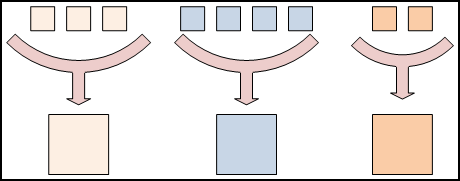
\includegraphics[width=5cm]{images/mapreduce}
  \end{column}
\end{columns}



\end{frame}


\subsection{Q\&A}

\begin{frame}
\centerline{Благодаря за вниманието!}
\end{frame}



\end{document}
